% This is samplepaper.tex, a sample chapter demonstrating the
% LLNCS macro package for Springer Computer Science proceedings;
% Version 2.21 of 2022/01/12
%
\documentclass[runningheads]{llncs}
%
\usepackage[T1]{fontenc}
% T1 fonts will be used to generate the final print and online PDFs,
% so please use T1 fonts in your manuscript whenever possible.
% Other font encondings may result in incorrect characters.
%
\usepackage{graphicx}
\usepackage{amsmath}
\usepackage{amssymb}
\usepackage{listings}
\usepackage{xcolor}
\usepackage{listings}
\usepackage{pgfplots}
\usepackage{array}
\usepackage{booktabs}
\usepackage{tikz}
% Used for displaying a sample figure. If possible, figure files should
% be included in EPS format.
%
% If you use the hyperref package, please uncomment the following two lines
% to display URLs in blue roman font according to Springer's eBook style:
%\usepackage{color}
%\renewcommand\UrlFont{\color{blue}\rmfamily}
%\urlstyle{rm}
%
\usetikzlibrary{shapes.geometric, arrows}
\tikzstyle{startstop} = [rectangle, rounded corners, minimum width=3cm, minimum height=0.6cm,text centered, draw=black, fill=red!30]
\tikzstyle{process} = [rectangle, minimum width=4cm, minimum height=0.8cm, text centered, draw=black, fill=orange!30]
\tikzstyle{decision} = [diamond, minimum width=3cm, minimum height=0.4cm, text centered, draw=black, fill=blue!30]
\tikzstyle{arrow} = [thick,->,>=stealth]

\lstdefinelanguage{solidity}{
  backgroundcolor=\color{pink!20},
  keywords={contract, function, public, int},
  keywordstyle=\bfseries\color{blue},
  commentstyle=\itshape\color{green!40!black},
  basicstyle=\ttfamily,
  morecomment=[l]{//},
  morecomment=[s]{/*}{*/},
  morestring=[b]",
  sensitive=true
}
\begin{document}
%
\title{Gas-Efficient Parameter Verification for Blockchain Smart Contracts Using Off-Chain Validators}
%
\titlerunning{Off-Chain Parameter Verification Approach: Gas-Efficient}
% If the paper title is too long for the running head, you can set
% an abbreviated paper title here
%
\author{Thi Thu Ha Doan\orcidID{0000-0001-7524-4497}\and Peter Thiemann\orcidID{0000-0002-9000-1239}}
%
\authorrunning{Ha Doan, P. Thiemann}
% First names are abbreviated in the running head.
% If there are more than two authors, 'et al.' is used.
%
\institute{University of Freiburg, Germany \\
  \email{\{doanha,thiemann\}@informatik.uni-freiburg.de}}
%
\maketitle              % typeset the header of the contribution
%
\begin{abstract}
In certain blockchain scenarios, verifying the properties of parameters may require significant gas costs or be infeasible due to gas limits. This study proposes a distributed verification protocol to address these challenges. The core concept involves offloading the verification process to validators, who attempt to find counterexamples or proofs off-chain. If a counterexample is discovered, it can be submitted for re-verification on-chain. If validated, the parameter is discarded; otherwise, the correctness of the parameter is guaranteed through a proof-of-work incentive mechanism, encouraging validators to participate in the distributed verification process. To implement these ideas, we propose a practical model that also tackles potential security concerns. We developed a prototype of the protocol and conducted a cost analysis, demonstrating its gas efficiency and practical utility.
\keywords{blockchain, off-chain verification, gas optimization, proof-of-work, distributed verification}
\end{abstract}
%
%
%
\section{Introduction}
\label{sec:introduction}
\lstset{language=solidity}
A smart contract is a critical component of blockchain technology, with applications ranging from simple tasks like auctions to more complex systems such as decentralized markets. However, broader adoption of smart contracts faces challenges, with gas costs being among the most significant. Every computation performed by a smart contract on the blockchain incurs a cost, as each unit of computation and storage consumed by an algorithm must be paid for due to the burden it places on the system \cite{eth-whitepaper,yellowpaper}.

When users (or other contracts) invoke a function in a smart contract, they must provide input data, known as parameters. In many cases, these parameters require verification. For instance, to minimize gas costs, an application might perform some computation off-chain and submit the result as a parameter to a smart contract. Such computations typically assert certain properties of the submitted parameters.

Another scenario involves interactions with external data sources. Since smart contracts cannot directly access off-chain data, blockchain oracles supply this information. When external data becomes available, an oracle invokes a smart contract with the relevant information.

However, while the contract should leverage off-chain computations or external data and assume that the submitted parameters are valid, there is a risk that off-chain computations could be incorrect, submitting invalid parameters, or that oracles could provide faulty data. Therefore, a mechanism is needed to verify these assumptions before the contract begins execution.

Unfortunately, most current applications cannot efficiently verify complex parameters on-chain due to the high gas costs associated with such computations. This limitation restricts many applications that require parameter verification during smart contract execution. The primary goal of this paper is to propose an approach that validates complex parameter assumptions while minimizing gas costs, without sacrificing computational efficiency.

Consider a contract that takes a prime number as a parameter:
\begin{lstlisting}[numbers=none]
contract Example {
  function (int p) public {
    // assume p is prime 
  ... }
}
\end{lstlisting}
This assumption can be expressed as an explicit assertion in predicate logic:
\begin{gather*}
\label{eq1}
  (\forall n) (2 \leq n \leq \sqrt{p}) \Rightarrow (p \mathbin{\%} n) \ne 0
\end{gather*}
Checking the validity of this assumption requires a loop in the contract. The test would take \(O(\sqrt{p})\) time (assuming constant time for computing the remainder) and produce extra cost linear in \(\sqrt{p}\).

Similarly, consider a contract that requires a sorted array of integers as input:

\begin{lstlisting}[numbers=none]
contract Sorted {
  function find (int[100] a, int v) public {
    // assume a is sorted 
  ... } 
}
\end{lstlisting}
The explicit assertion would be:
\begin{gather*}\label{}
  (\forall k) (0\leq k <99) \Rightarrow a[k] \leq a[k+1]
\end{gather*}
This check can be performed in \(O(1)\) time, but the associated constant factor makes it costly.

However, we could do better by recruiting the validators of the contract for a distributed effort to find a counterexample off-chain. To this end, we consider the negation of these assertions. 

For the prime number example, the negation is:
\begin{gather*}\label{}
  (\exists n) (2 \leq n \leq \sqrt{p}) \wedge (p \mathbin{\%} n) = 0
\end{gather*}
This assertion can be checked pointwise by having each validator independently choose a random \(n\) fulfilling \(2 \leq n \leq \sqrt{p}\) and checking whether \((p \mathbin{\%} n) = 0\). If the remainder is \(0\), the validator has found a counterexample and submits its veto to the on-chain contract, which then verifies the counterexample. If valid, the contract halts further execution with that parameter. If no counterexample is found, \(p\) is accepted, assuming other validators have checked other points.

For the sorted array example, the negation is:
\begin{gather*}\label{}
  (\exists k) (0\leq k <99) \wedge a[k] > a[k+1]
\end{gather*}
Again, we can have every validator generate a random number \(k\). If the condition is true for such \(k\), the validator has found a counterexample for the sortedness of the array. Otherwise, the validator relies on others to check different indices.

Instead of looping and checking all points on-chain, only one or some points are checked. The checking process can be performed off-chain with no gas cost, and only the result of the verification process needs to be validated on-chain. By shifting much of the verification off-chain, our propsed approach significantly reduces gas costs, as only counterexample verification occurs on-chain.

This approach substantially reduces on-chain gas costs by moving most of the verification work off-chain. However, it introduces challenges related to incentivizing validators, ensuring the cost-effectiveness of on-chain verifications, and providing correctness guarantees when no counterexamples are found.

To address these challenges, we propose a proof-of-work-based incentive mechanism that encourages validator participation and ensures that parameters meet the desired properties with a high level of confidence. The detailed methodology of this approach are discussed in Section \ref{sec:offchain-distributed-verification-approach}.

To realize our novel approach, we propose a practical model that implements the approach and addresses security concerns. We then develop a prototype of the practical model for a decentralized marketplace application using Solidity on the Ethereum blockchain.

The contributions of this paper include:
\begin{itemize}
    \item A novel approach for verifying computationally expensive parameters (in terms of gas cost) for smart contracts on the blockchain.
    \item A proof-of-work-based incentive mechanism that motivates validators to participate in the distributed verification process and ensures the correctness of the submitted parameter with a high expected probability.
    \item A practical model that realizes the proposed novel approach, along with a prototype implementation of the model for a Solidity smart contract application on the Ethereum blockchain.
\end{itemize}


The paper is structured as follows: The next section defines the parameter verification problems and presents use cases. Section \ref{sec:offchain-distributed-verification-approach} proposes the novel approach, while Section \ref{sec:practical-model} introduces its practical model. Section \ref{sec:gas-cost-analysis} analyzes the gas costs, comparing our proposed approach with the on-chain method. Section \ref{sec:prototype-implementation} details the prototype implementation. Section \ref{sec:related-work} discusses related work, and Section \ref{sec:conclusion} concludes the paper.
\section{Parameter Assertion Verification On-chain}
\label{sec:parameter-assertion-verification-onchain}
Our work focuses on parameters that are computationally expensive to verify on-chain. Specifically, we address cases where verifying a parameter assertion requires loops within the contract and the assertion can be formalized using universal or existential quantifiers.
\subsection{Parameter Assertion Formalization}
\paragraph{Universal Quantifier Formalization}
An assertion can be formalized using the universal quantifier as follows:
\begin{gather}
  \label{eq:1}
  \forall a \in A. \, P(a)
\end{gather}
This formula can be extended to assertions over multiple domains as:
\begin{gather}
  \label{eq:2}
  \forall a \in A, \, \forall b \in B, \, \dots \, P(a, b, \dots)
\end{gather}
\paragraph{Existential Quantifier Formalization}
In cases where an assertion involves the existence of an element, it can be formalized using existential quantifiers as follows:
\begin{gather}
  \label{eq:3}
  \exists a \in A. \, P(a)
\end{gather}
This formula can also be extended to assertions over multiple domains:
\begin{gather}
  \label{eq:4}
  \exists a \in A, \, \exists b \in B, \, \dots \, P(a, b, \dots)
\end{gather}
\subsection{On-chain Verification}
Verifying these assertions on-chain requires iterating over the domain \(A\) within the contract. For the fomulas \ref{eq:5}, the verification fomulas is as follows.
\begin{gather}
  \label{eq:5}
  \bigwedge_{a \in A} P(a)
\end{gather}
For multiple domains, the verification process becomes:
\begin{gather}
  \label{eq:6}
  \bigwedge_{a \in A, b \in B, \dots} \dots P(a, b, \dots)
\end{gather}
Verifying these assertions in  the existential quantifier formalization requires iterating over the domain \(A\) until finding an element \(a\) that satisfies the predicate:
\begin{gather}
  \label{eq:7}
  \bigvee_{a \in A} P(a)
\end{gather}

For multiple domains, the verification process becomes:
\begin{gather}
  \label{eq:8}
  \bigvee_{a \in A, b \in B, \dots} \dots P(a, b, \dots)
\end{gather}
When the domain \(A\) is large or the predicate \(P\) is complex to evaluate, performing the verification on-chain incurs significant gas costs or even make the verification process infeasible due to gas limits. Given the current high gas prices, this can result in substantial costs.
\subsection{Use Cases}
Smart contract languages like Solidity, Vyper, Michelson, and Plutus support common data types such as numbers, booleans, strings, bytes, arrays, sets, and maps. Many properties of these types can be expressed using universal quantifiers, requiring loops for verification in smart contracts, but can often be disproven by a counterexample or proven with a proof. Below are key properties for each type:
\paragraph{\textbf{Numbers}}
Number types exhibit some properties that are crucial in cryptographic applications, such as primality and coprimeness. For example, the condition for two numbers \(a\) and \(b\) to be coprime is:
\begin{gather*}
\label{}
(\forall n \in \mathbb{N}) \ (2 \leq n \leq \min(a, b)) \Rightarrow \neg((a \mod n = 0) \wedge (b \mod n = 0))
\end{gather*}
\paragraph{\textbf{Booleans}}
SAT problems involve determining if there exists an assignment of variables that makes a formula \( F \) in propositional logic true. Verifying if a given assignment satisfies a formula \( F \), which is usually in Conjunctive Normal Form (CNF), requires looping over variables and clauses. Although finding a satisfying assignment is NP-complete, verifying an assignment takes \( O(n \times m) \), where \( n \) is the number of clauses and \( m \) is the number of variables.
\paragraph{\textbf{Strings}}
String properties that require iteration include uniqueness (no repeated characters), character set membership, lexicographical order, pattern matching, and forbidden substrings. For instance, verifying that a string \(s\) does not contain a forbidden substring \(f\) of length \(k\) can be expressed as:
\begin{gather*}
(\forall i) \ (0 \leq i \leq n - k) \Rightarrow s[i, i+1, \dots, i+k-1] \neq f
\end{gather*}
\paragraph{\textbf{Bytes}}
Verifying byte arrays often requires loops for properties like uniformity, sorted order, specific byte patterns, uniqueness, valid range, and alternating patterns. For example, to check if all bytes in an array \(b\) lie within a range \([l, u]\), the condition is:
\begin{gather*}
(\forall i) \ (0 \leq i \leq n) \Rightarrow l \leq b[i] \leq u
\end{gather*}
\paragraph{\textbf{Arrays (or Lists)}}
Common properties of arrays include sortedness, uniqueness, boundedness, monotonicity, symmetry, cyclic structure, and constant values. %A tree-based structure like a max-heap, where each parent node is greater than or equal to its children, can be checked as:
Tree-based structures like heaps can also be built from arrays, with properties such as the heap property. For example, in a max-heap, each parent node is greater than or equal to its children. This property can be expressed as:
\begin{gather*}
(\forall i) \ a[i] \geq a[2i+1] \land a[i] \geq a[2i+2]
\end{gather*}
\paragraph{\textbf{Sets}}
Set properties like subset verification, disjoint sets, element uniqueness, set equality, and set intersection often require loops. For example, verifying that two sets \(A\) and \(B\) share at least one element can be expressed as:
\begin{gather*}
(\exists a \in A) (\exists b \in B)\ a = b
\end{gather*}
Such properties can be computationally expensive for large sets.
\section{Off-chain Distributed Verification Approach}
\label{sec:offchain-distributed-verification-approach}
\subsection{The Outline of the Approach}
We propose a novel approach for verifying parameter assertions in blockchain-based smart contracts. Our approach distributes the verification process off-chain, submitting only the outcomes to the blockchain for re-verification. This strategy aims to significantly reduce the computational burden on the blockchain while maintaining the integrity of the contract.

Our approach takes into account the key principle that assertions expressed with universal quantifiers can be disproven by counterexamples, while those with existential quantifiers can be proven with valid proofs. These counterexamples or proofs serve as checkpoints, representing specific elements within the domain. 

The outline of our approach is as follows:
\paragraph{\textbf{Determine the checkpoint formula.}}
The first step is to establish the checkpoint formula used to identify counterexamples or proofs. For assertions with universal quantifiers, as shown in Equation~\ref{eq:1}, the checkpoint formula is the negation of the original assertion and is expressed using an existential quantifier as follows: 
\begin{gather}
\label{eq:9}
(\exists a \in A) \ \neg P(a)
\end{gather}
For assertions over multiple domains, as in Equation~\ref{eq:2}, the checkpoint formula becomes:
\begin{gather}
\label{eq:10}
(\exists a \in A) (\exists b \in B) \dots  \neg P(a, b, \dots)
\end{gather}
In the case of existential quantifier assertions, as in Equation~\ref{eq:3} and Equation~\ref{eq:4}, the checkpoint formula remains the same as the original assertion.
\paragraph{\textbf{Off-chain distributed effors.}}These checkpoint formulas are then distributed to validators. Off-chain, the validators attempt to find counterexamples or proofs by identifying some \( a \in A \) such that the checkpoint formula is satisfied. For universal quantifier formalizations, this means finding \( a \) where \( \neg P(a) \) holds, and for existential quantifier formalizations, finding \( a \) where \( P(a) \) is true.
\paragraph{\textbf{On-chain re-verification.}} Once a counterexample or proof involving an element \( a \) is found, the validator submits it to the blockchain, where it is re-verified by evaluating \( \neg P(a) \) or \( P(a) \) on-chain. For assertions with universal quantifiers, when a counterexample is successfully verified on-chain, the parameter assertion is proven to be invalid. Otherwise, it is considered valid, assuming that other points are checked by other validators. For assertions with existential quantifiers, the parameter assertion remains invalid until a proof is submitted and successfully re-checked on-chain.
\paragraph{\textbf{Incentivization Mechanism.}} Validators are incentivized to find counterexamples or provide proofs, which require computational resources. Since counterexamples are rare (as callers avoid submitting invalid parameters), confidence in correctness grows with more validator attempts at different checkpoints. Thus, incentivization is crucial for ensuring correctness in the absence of counterexamples.Validators are rewarded for both finding counterexamples and contributing computational proofs, with  counterexample discovery prioritized through higher rewards. 

This approach reduces the blockchain's burden and lowers gas costs by verifying only specific checkpoints, rather than performing full on-chain verification.
\subsection{Proof-of-Work-Based Incentivization Mechanism}
The computational effort is represented by a computation proof, which is then submitted on-chain by the validator to claim their reward. This approach encourages participation in the distributed verification process, ensuring thorough validation even without the discovery of counterexamples.

However, significant challenges arise regarding (1) how to recheck the counterexample and the computation efforts on-chain at a reasonable gas cost, (2) how to ensure a significant number of checkpoints have been performed before a computation reward is issued, in order to guarantee an expected probability of correctness for the parameter, and (3) how to ensure that validators actually perform the checkpoint formula off-chain when no counterexample is found but a computation reward is provided.

To overcome these challenges, we propose a proof-of-work-based incentivization mechanism. We utilize the proof-of-work concept by introducing a target hash \( t \), which sets the required difficulty level to earn the computation reward. The basic idea is that each verification process introduces a target hash. The validator attempts to perform the negation check and compute a hash that is less than or equal to the given target hash. The objective of the validator is to find either a counterexample or a computation that produces a hash smaller than or equal to the target hash \( t \).
\subsubsection{Introduce a seed} To recheck the counterexample or computation proof on-chain at a reasonable gas cost, the counterexample or computation proof should be submitted on-chain in the form of the indication of the element \( a \in A \) where the assertion is invalid, in the case of a counterexample. The on-chain re-verification process is then straightforward, simply requiring the evaluation of \( \neg P(a) \).

The next challenge is how to generate a random hash for each computation and devise a computational proof to incentivize computational effort. To address this, we introduce a seed \( s \) in each verification process.

Let \( n \) denote the size of the domain \( A \). 
\begin{gather*}
n = |A|
\end{gather*}
where \(|A| \) denotes the number of elements in the domain $A$.

Each number \( i \) in the range \([1, n]\) corresponds to an element in \( A \). 
\begin{gather*}
a=A[i]
\end{gather*}
where $A[i]$ denotes the $i$-th element in $A$.

The seed \( s \) is a random number. 
\begin{gather*}
s \in \mathbb{N} 
\end{gather*}
The seed $s$  is then reduced with modulo \( n \) to obtain \( i \), which is associated with an element \( a \) in \( A \).
\begin{gather}
\label{eq:11}
i = (s\mod n) + 1
\end{gather}
\subsubsection{Estimate the number of seeds:} To ensure that a sufficient number of checkpoints have been checked before a computational proof is found, we first estimate the number of seeds required to find a counterexample with the desired probability of correctness.

Assuming the unsatisfied element is only the first element \( a_0 \) in \( A \) and the number of seeds is \( m \), each seed independently has a probability of \( \frac{1}{n} \) to detect the issue and \( \frac{n-1}{n} \) not to. If each seed associated with an element \( a \) in \( A \) is chosen uniformly and independently, the probability that no seed checks \( a_0 \) approaches 0 as \( m \) increases:
\begin{gather*}
\lim_{m \to \infty} \frac{(n-1)^m}{n^m} = \lim_{m \to \infty} \left( \frac{n-1}{n} \right)^m = 0
\end{gather*}

To determine the number of seeds needed based on the expected probability of detecting a problem, we define \( p \) as the expected probability of finding at least one counterexample. 
\begin{itemize}
    \item The probability of a single seed failing to find a counterexample is \( \frac{n-1}{n} \).
    \item The probability of all \( m \) seeds failing is \( \left( \frac{n-1}{n} \right)^m \).
    \item Thus, the probability of at least one seed finding a counterexample is:
\begin{gather*}
  p = 1 - \left( \frac{n-1}{n} \right)^m
\end{gather*}
\end{itemize}
%Rearranging this gives:
%\begin{gather*}
%\left( \frac{n-1}{n} \right)^m = 1 - p
%\end{gather*}
%Taking the natural logarithm:
%\begin{gather*}
%m \ln\left( \frac{n-1}{n} \right) = \ln(1 - p)
%\end{gather*}
Solving for \( m \):
\begin{gather}
\label{eq:12}
m = \frac{\ln(1 - p)}{\ln\left( \frac{n-1}{n} \right)}
\end{gather}

So the number of the seeds to achive the expected propety $p$ is great or at least equal to $m$. Note that, \( p \) represents the probability when only one validator participates. As more validators are involved, the probability of discovering a counterexample increases.
\subsubsection{Set up the taget hash:}
The above number of seed $m$ can then be used to set up the target hash $t$. The target hash $t$ can be calculated based on a desired difficulty level. In proof-of-work systems, difficulty is typically adjusted to ensure that the average efforts to find a valid hash. The target hash $t$ is often calculated by taking the maximum possible hash value and dividing it by the difficulty level.

Given the expected number of seeds to generate, 
the difficulty level \( D \) can be adjusted accordingly. Typically, \( D \) is set to ensure that a valid hash is found approximately once every \( m \) trials.

If we want the probality of finding a valid hash to be $\frac{1}{m}$, then \( D \) equal to \( m \):
\begin{gather}
\label{eq:13}
t = \frac{H_{\text{max}}}{m}
\end{gather}

Where \( H_{\text{max}} \) is the maximum possible hash value and \( m \) is the difficulty level, which can be adjusted based on the expected number of trials.
\subsubsection{Conduct a Computation Hash:} To ensure that a computational proof includes the negation check, the computation of the checkpoint formula is integrated into the proof process. This guarantees that validators must execute the negation check as part of producing the computation proof.

For each element \( a \), let \(\pi_{P_{a}}\) be the function that returns the essential components of evaluating the negation \(\neg P(a)\). The computation hash thus incorporates both the seed \( s \) and \(\pi_{P_{a}}\), ensuring proper validation.

\begin{gather}
\label{eq:14}
t_s = \text{hash}(s, \pi_{P_{a}})
\end{gather}
where \(\text{hash}\) is a cryptographic hash function used to compute the hash value.

Assertions in smart contract languages, such as Solidity and Michelson, are often represented as predicate logic, expressed through Boolean formulas. These are composed of relational operators like \( =, \neq, >, <, \geq, \leq \), logical operators such as \( \neg, \land, \lor\), and corresponding expressions.

Thus, \(\pi_{P_{a}}\) represents the set of expressions involved in evaluating the predicate \(P_a\).
\begin{gather*}
\pi_{P_{a}} = \{ e_1, e_2, \ldots \}
\end{gather*}
where \(e_i\) are the expressions that contribute to the computation of the predicate \(P_a\).


%For example, for each element \( i \), it returns \(a[i]\) and \(a[i + 1]\) in the evaluation of the negation predicate \( a[i] < a[i+1] \) in the sorted array example.

%The expressions $\pi_{P_a}$ can be used to compute the hash, which involves the validator executing the condition check to find a reward computation.
%\begin{equation}
%t_s = \text{hash}(s, \pi_{P_{a}})
%\end{equation}
%where:
%\begin{itemize}
%    \item $s$ is the seed.
%    \item $\pi_{P_{a}}$ is the set of expressions used in the computation of the predicate $P_a$.
%    \item \text{hash} is the hash function that computes the hash based on the seed and the set of expressions $\pi_{P_{a}}$.
%\end{itemize}
\subsection{Off-chain distributed verification}
For applications where the parameter assertion can be expressed using an existential quantifier, the validation process is relatively straightforward. Validators attempt to find a proof off-chain and submit it on-chain, where it is re-verified. If the proof is valid, the parameter is considered correct, and the validator is rewarded.

However, for assertions involving universal quantifiers, the process becomes more complex. First, the size \( n \) of the domain \( A \) is calculated. Then, using the expected probability to ensure the correctness of the parameter assertion in the absence of a counterexample, the target hash is computed. Due to the setup of the target hash, a validator needs to generate approximately \( m \) seeds to have a chance of discovering either a counterexample or a computational proof, thereby confirming the validity or revealing the invalidity of the parameter.

The process of finding a valid seed is outlined in Fig. \ref{fig:find_seed}. During this distributed process, each validator generates a seed \( s \) and performs the negation check until they either identify a counterexample or a computation proof for a reward. Once one of these outcomes is achieved, the validator can submit it on-chain to claim their reward.

Both the counterexample and the computational proof are encoded by the seed, allowing the on-chain component to replicate and verify the result. If the verification is successful, the validator receives the reward.
\begin{figure}[t]
    \centering
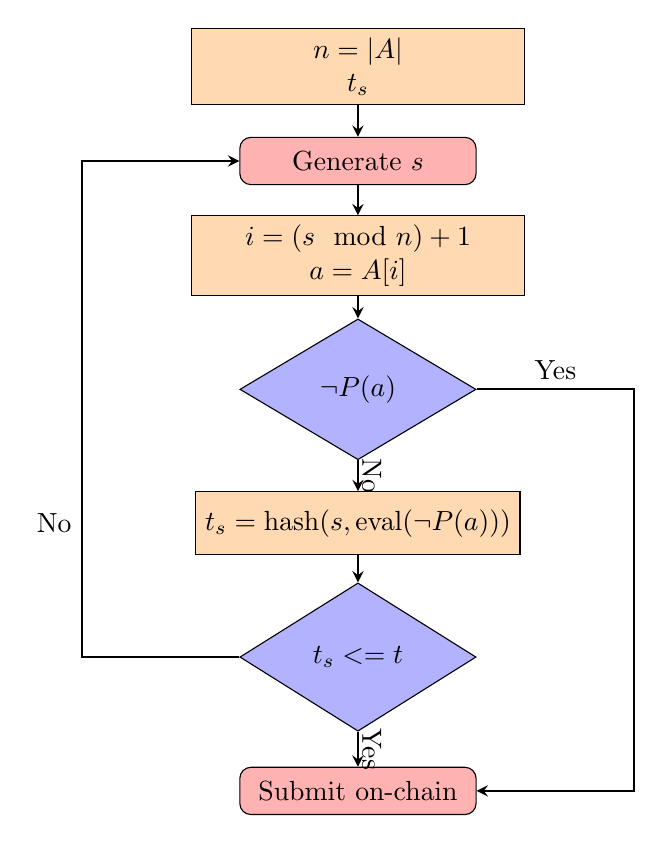
\begin{tikzpicture}[node distance=1.2cm]
    % Nodes
    \node (calc_n) [process] {\parbox{4cm}{\centering $n = |A|$ \\ $t_s$}}; 
    \node (start) [startstop, below of=calc_n] {Generate $s$};
    \node (calc_i) [process, below of=start] {\parbox{4cm}{\centering $i = (s \mod n) + 1$ \\ $a = A[i]$}};
    \node (counterexample) [decision, below of=calc_i, yshift=-0.5cm] {$\neg P(a)$};
    \node (calc_hash) [process, below of=counterexample, yshift=-0.5cm] {$t_s = \text{hash}(s, \text{eval}(\neg P(a)))$};
    \node (compare) [decision, below of=calc_hash, yshift=-0.5cm] {$t_s <= t$};
    \node (submit) [startstop, below of=compare, yshift=-0.5cm] {Submit on-chain};
    % Arrows
    \draw [arrow] (calc_n) -- (start);
    \draw [arrow] (start) -- (calc_i);
    \draw [arrow] (calc_i) -- (counterexample);
    \draw [arrow] (counterexample) -- node[midway, above, sloped, anchor=center, yshift=0.5em] {No} (calc_hash);
    \draw [arrow] (calc_hash) -- (compare);
    \draw [arrow] (compare) -- (submit) node[midway, above, sloped, anchor=center, yshift=0.5em] {Yes};
	\draw [arrow] (counterexample.east) -| node[pos=0.25, above] {Yes} ([xshift=2cm]submit.east) |- (submit);
	\draw [arrow] (compare.west) -| node[pos=0.75, left] {No} ([xshift=-2cm]counterexample.west) |- (start);
\end{tikzpicture}
\caption{Finding a reward seed.}
\label{fig:find_seed}
\end{figure}
\subsection{On-chain re-verification}
Given a submitted seed \( s \), the on-chain contract verifies whether the seed produces a counterexample or a valid computational proof eligible for a reward. The verification process follows these steps:
\begin{enumerate}
    \item Compute \( n \), the size of the domain \( A \).
    \item Identify the target value \( t \).
    \item Determine \( i \in [1, n] \) from \( s \) using the modulo operation, and associate \( i \) with the corresponding element \( a \) in \( A \).
    \item Perform the check \( \neg P(a) \) to see if \( a \) is a counterexample.
    \item If no counterexample is found, compute the hash \( t_s \) derived from the seed \( s \).
    \item Compare \( t_s \) to the target hash \( t \) to check if it qualifies for a reward.
\end{enumerate}

Following this process, the contract will either identify a counterexample or compute a hash based on the seed \( s \) and the evaluation \( \neg P(a) \). The computed hash is then compared to the target hash to determine if it qualifies for a reward. The possible outcomes are: finding a counterexample, validating a reward computation, or determining no reward computation.
\section{Practical Model}
\label{sec:practical-model}
\subsection{Security risks}
Off-chain distributed verification of assertions is indeed an intriguing concept, yet it faces the following security risks when proposing an incentive method:

\begin{enumerate}
\item Denial-of-service (DoS) attacks: The system is susceptible to DoS attacks, where a caller inundates the system with numerous invalid parameters, causing congestion and hindering its operation.
\item Front-running attacks: The system is vulnerable to front-running attacks, where an attacker closely monitors the mempool to intercept a seed representing a counterexample or a computation proof, subsequently stealing the reward.
\item Caller exploitation: A caller might exploit the system by running the negation check privately to (1) identify the reward before submitting the parameter on-chain, thereby swiftly claiming the reward ahead of the other validators, (2) fake the compuatation proofs before a counterexample can be found by other validators.
\item Reward manipulation: For a system that allows multiple rewards. A validator may attempt to manipulate the reward system by resubmitting counterexamples or computation proofs multiple times to multiply their rewards.
\end{enumerate}
\subsection{Overview architect}
This section presents a practical model that unifies theoretical principles and addresses the previously mentioned security concerns. The architectural design of this model is depicted in Figure \ref{fig.architect}.  
\subsubsection{Main compoments.} The model consists of two main entities: the on-chain assertion contract and the off-chain validator program.
\paragraph{On-chain assertion contract.}
While additional functions may exist, the assertion contract must encompass the following two essential functions (or similar functions):
\begin{itemize}
\item The \( submitParameter \) function: Callers utilize this function to submit their parameters for validation. %Subsequently, the parameter is distributedly verified by validators.
\item  The \( claimReward \) function: This function accepts a seed (or may some others) as inputs, yielding a result indicating whether the computation from the seed results in a counterexample, a reward computation, or a non-reward computation.
\end{itemize}
\paragraph{Off-chain validator program.}
Since the off-chain program runs off-chain, it can be implemented according to the validator's preferences. However, the crucial point is that the off-chain contract must use the exact same \( claimReward \) function when attempting to find a counterexample or a computation proof. Additionally, it should support a function that assists the validator in finding a seed to earn a reward.

All events such as parameter submissions, the discovery of a counterexample, or the presentation of computational proofs can be broadcasted to the network using event emission. Validators can monitor these events to stay updated on the verification status in real-time.
\paragraph{Storage.}
When a parameter is submitted for verification, the following information should be stored:
\begin{itemize}
\item Parameter: this includes the parameter itself. In cases where storing the parameter on-chain is impractical because of its size, it could be possible to store only its hash. Despite this, the hash remains sufficient for validation.
\item Timestamp: this indicates the approximate time when the parameter was submitted.
\end{itemize}
\begin{figure}
\centering
\includegraphics[scale=.8]{assertion1}
\caption{The architecture of the practical model}
\label{fig.architect}
\end{figure}
\subsubsection{Deploying and managing on/off-chain contracts.}
The respective owner is responsible for deploying the on-chain contract and ensuring that the off-chain program is accessible to validators. There are two approaches to make the program available to validators:
\begin{itemize}
   \item The owner may store the program code in a repository that is accessible to validators or provide it directly to them upon request. 	\item Alternatively, the owner can broadcast the program to the network using messaging systems like Waku in Ethereum, allowing interested validators to store the off-chain code locally.
\end{itemize}

%\subsubsection{On and Off.} 
%Before a parameter can be utilized in the actual work function or contract, a caller must initially submit it via the submit-parameter function in the on-chain assertion contract. 

%Upon the submission of a parameter, an event can be emitted, allowing validators to receive updates by monitoring the blockchain for the parameter submission event. Additionally, the caller may choose to broadcast their parameter to all validators via a messaging system when submitting it online.
%\subsubsection{Off-chain verification}
%After a parameter is submitted and stored on-chain, a validator can commence the verification process. To assess the validity of a parameter, each validator independently executes the off-chain validation program.

%A validator may attempt to try multiple times with different random seeds in order to find either a counterexample or a computational proof. A function called find-seed could be implemented, which in turn calls the claim-reward function to locate a seed.

%All events such as parameter submissions, the discovery of a counterexample, or the presentation of computational proofs can be broadcasted to the network using event emission. Validators can monitor these events to stay updated on the verification status in real-time. 
\subsubsection{Calling a work function}
A work function can be encapsulated as a private function within the assertion contract or implemented in a separate contract. A caller submits a parameter for verification through the on-chain assertion contract. Once verified, the work contract is triggered to perform its task under the assumption that the parameter is valid.

The work function or contract is invoked by the on-chain validation contract or caller, but only if specific conditions are met, such as sufficient verification proofs, no counterexamples, and a waiting period. Upon fulfilling all requirements, the task is executed, and in some cases, the parameter record may be deleted to free up storage.
\subsection{Security Features}
\subsubsection{DoS attacks}
When submitting a parameter, the caller must provide a deposit in native tokens. This deposit is claimed by a validator if a counterexample is found or returned if the parameter is verified. The deposit discourages invalid submissions and mitigates the risk of DoS attacks.
\subsubsection{Front-running attacks}
To prevent front-running attacks, the seed \( s \) is calculated by combining a random number \( r \) with the validator's address, rather than using \( r \) alone. This approach enhances security, as a malicious validator cannot reuse \( r \) from the mempool - its combination with their own address will yield a different seed \( s \).

%While a random number $r$ alone as a seed is sufficient to indicate the associated element $a$ in the domain $A$, to prevent the front-running attack, we enhance the randomness of the seed by combining a random number with the validator's address to calculate the seed.

%This combination adds an extra level of security. So even watching the mempool and get the random number, a malicious validators cannot use the same random number $r$  because the combination with their address will not produce the same seed $s$.

 %In deeds, the validator's address is converted to numerical values and use these numbers in combination with a random number to compute the seed. 

%Let's denote the validator's address by $addr$: \(\quad \text{addr} \in \text{Addresses}\)

%The address is converted to numerical values.
%\begin{equation}
%\text{addr\_num} = \text{init256}(\text{addr})
%\end{equation}


%This combination adds an extra level of security. So even watching the mempool and get the random number, a malicious validators cannot use the same random number $r$  because the combination with their address will not produce the same seed $s$.
\subsubsection{Caller exploitation attack}
%A caller may execute the validator program for their parameters before submitting on-chain, attempting to claim a reward or validate their parameter before others find counterexamples.
To mitigate the caller exploitation risk, the seed \( s \) is computed using the block timestamp \( t \) indicating when the parameter is submitted, random number \( r \), and validator's address. The timestamp \( t \in \text{Timestamps} \) is included to prevent preemptive submission, and the seed \( s \) is calculated as:
\begin{equation}
s = \text{hash}(r, \text{addr}, t)
\end{equation}
where \(\text{hash}\) is a cryptographic hash function. This ensures that manipulated or pre-run seeds fail to produce counterexamples or rewards.
%Additionally, applications can enforce a time frame such that a parameter is valid only if enough time has passed for verification. A parameter is valid if, after this time, no counterexample is found and sufficient computation proofs are received.
\subsubsection{Reward manipulation attack}
In some applications, multiple computational proofs are allowed, and a record is maintained to track the parameter's verification progress. This record contains validator addresses and the random number \( r \) used in each verification. 

The inclusion of validators' addresses and \( r \) is crucial in preventing reward manipulation, as it ensures that a validator cannot resubmit with the same \( r \), thereby preventing repeated claims for the same computation proof or counterexample.
\section{Gas Cost Analysis}
\label{sec:gas-cost-analysis}
This section evaluates the cost of the proposed distributed verification method and compares it to traditional on-chain verification.
\subsection{Transaction Execution Costs}
Transaction costs, measured in gas, can be divided into five key components:
\begin{enumerate}
\item Base cost: Fixed cost for initiating a transaction, covering operations like hashing, signature verification, and balance updates. For instance, transferring ETH in Ethereum costs 21,000 gas.
\item Data cost: Gas tied to the size of the transaction’s data payload, with non-zero bytes incurring higher costs than zero bytes.
\item Computational cost: Gas for executing smart contract operations, such as arithmetic, logic, control flow, cryptography, and memory tasks.
\item Storage cost: Higher than computation, as it involves writing to persistent storage. %In Ethereum, writing a new value costs 20,000 gas, updates cost 5,000 gas, and reading costs 100 gas.
\item Refund gas: Gas refunded for specific operations, like using SELFDESTRUCT or resetting storage values to zero.
\end{enumerate}
Thus, the total gas cost (execution cost) includes base, data, computational, and storage costs.
\subsection{Comparative Analysis of On-Chain and Offline Distributed Methods}
We compare the gas costs of on-chain and off-chain verification by breaking down their components.
\subsubsection{On-chain Verification Gas Costs}
Let \( G_{parameter} \) represent the intrinsic gas cost, which includes base and data costs, primarily depending on the size of the parameter \( p \). The total on-chain gas cost \( G_{on} \), given in Equation \ref{on-gas}, includes:
\begin{itemize}
    \item Intrinsic gas \( G_{parameter} \),
    \item Optional storage gas \( G_{storage} \),
    \item Gas for \( n \) parameter checks, each costing \( G_{check} \),
    \item Execution gas \( G_{run} \), if the parameter is valid.
\end{itemize}
\begin{equation}
\label{on-gas}
G_{on} = G_{parameter} + [G_{storage}] + n \cdot G_{check} + G_{run}
\end{equation}

\subsubsection{Off-chain Verification Gas Costs}
The off-chain verification gas costs include similar components to on-chain verification but differ in several key aspects. Instead of \( n \) parameter checks, only a single check is required. Moreover, storage cost \( G_{storage} \) is mandatory, and additional components are needed as follows:
\begin{itemize}
    \item Submit the seed, \( G_{seed} \),
    \item Compute and compare the hash, \( G_{hash} \).
\end{itemize}
The total off-chain gas cost is given by Equation \ref{gas-off}:
\begin{equation}
\label{gas-off}
G_{off} = G_{parameter} + G_{storage} + (G_{seed} + G_{check} + G_{hash}) + G_{run}
\end{equation}

\subsubsection{Comparative Analysis}
We compare the gas costs of both verification methods.
Both methods incur the same intrinsic cost, \( G_{parameter} \).
On-chain storage cost \( [G_{storage}] \) is optional, whereas the offline method always includes \( G_{storage} \), which may store only the parameter's hash. The on-chain method incurs \( n \cdot G_{check} \) for parameter checking, while the offline method reduces this to \( G_{check} \). The offline method includes costs for seed submission \( G_{seed} \) and hash computation \( G_{hash} \), which are not required for the on-chain method. Finally, both methods share the computation cost, \( G_{run} \).

Define \( G_{base} \) as the sum of submission, storage, and computation costs:
\[
G_{base} = G_{parameter} + [G_{storage}] + G_{run}
\]

The offline distributed process uses a proof-of-work incentive; let \( G_{reward} \) be the gas equivalent reward for counterexamples or proofs. The total verification cost for proof \( G_{proof} \) is:
\[
G_{proof} = G_{seed} + G_{check} + G_{hash} + G_{reward}
\]

Figure \ref{fig:gas_compare} compares gas consumption between methods, with \( G_{base} \) assumed constant. The red line (on-chain) scales linearly with parameter size \( n \), while the blue line (offline) initially incurs higher costs but becomes more efficient as \( n \) grows.

The on-chain method is best for scenarios requiring direct blockchain checks, but it becomes costly when \( n \) and \( G_{check} \) are large. The proposed offline method (\( G_{off} \)) is more efficient for large parameters, despite additional \( G_{seed} \) and \( G_{hash} \) costs, which are often outweighed by savings in reduced checks.

For the offline method, the main concern is \( G_{storage} \). If storing the parameter is required, this cost is negligible, but if not, it must be considered, potentially storing only the parameter's hash for verification.

Overall, the offline method (\( G_{off} \)) is generally more cost-effective for large parameters, depending on \( n \), \( G_{storage} \), and specific values of \( G_{seed} \), \( G_{hash} \), and \( G_{reward} \).
\begin{figure}
  \centering
  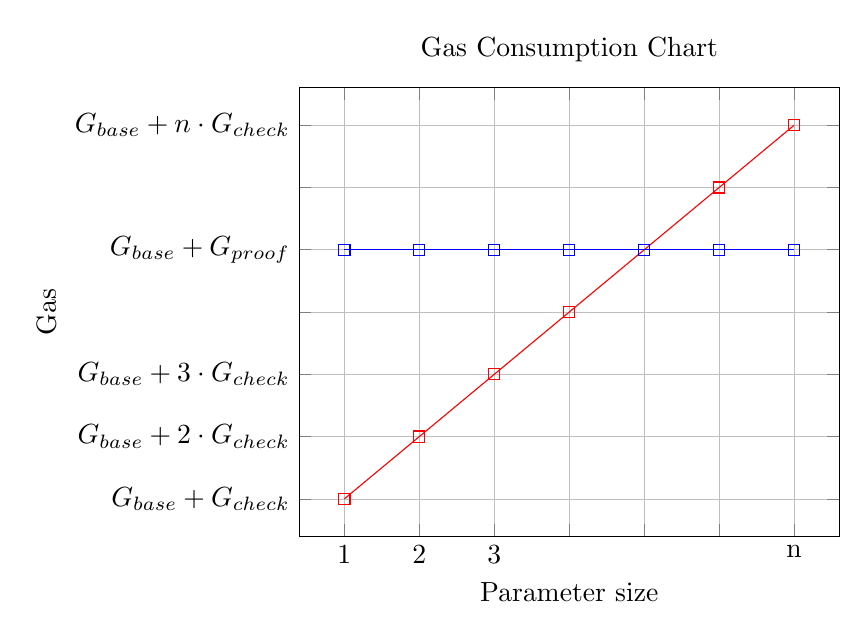
\begin{tikzpicture}
    \begin{axis}[
        title={Gas Consumption Chart},
        xlabel={Parameter size},
        ylabel={Gas},
        grid=both,
        major grid style={line width=.2pt,draw=gray!50},
        minor grid style={line width=.1pt,draw=gray!20},
        xtick={1,2,3,4,5,6,7,8},
        xticklabels={1,2,3,,,,n,},
        ytick={1,2,3,4,5,6,7,8},
        yticklabels={$G_{base} + G_{check}$,$G_{base} + 2 \cdot G_{check}$, $G_{base} + 3 \cdot G_{check}$,,$G_{base}+ G_{proof}$,,$G_{base} + n \cdot G_{check}$,},
    ]
      \addplot[
        color=red,
        mark=square,
        ]
        coordinates {
        (1,1)(2,2)(3,3)(4,4)(5,5)(6,6)(7,7)
        };
         \addplot[
        color=blue,
        mark=square,
        ]
        coordinates {
        (1,5)(2,5)(3,5)(4,5)(5,5)(6,5)(7,5)
        };
    \end{axis}
  \end{tikzpicture}
  \caption{Gas Cost Comparison}
  \label{fig:gas_compare}
\end{figure}
\section{Prototype Implementations}
\label{sec:prototype-implementation}
This section presents the implementation of the Decentralized Selling Platform (DSP) application. Initially, the DSP is deployed as a smart contract on the Ethereum blockchain, where parameter verification occurs on-chain. We then demonstrate how an off-chain verification approach can significantly reduce gas costs.
\subsection{Decentralized Selling Platform}
The DSP application provides a decentralized framework for managing and trading items. Sellers can create platforms, list items, and facilitate buyer transactions. Buyers can directly purchase items listed for sale.

Each item in the platform is characterized by:
\begin{itemize}
    \item \texttt{product}: A struct representing the product, including its name and producer.
    \item \texttt{forSale}: A boolean indicating whether the item is available for sale.
    \item \texttt{price}: The price of the item, specified in wei.
    \item \texttt{owner}: The Ethereum address of the current item owner.
\end{itemize}
The DSP application provides several key functions:
\begin{itemize}
    \item \texttt{createSellingPlatform(items)}: Creates a selling platform with a list of sorted items.
    \item \texttt{buyItem(sellingPlatform, product)}: Enables buyers to purchase an item if listed for sale at the correct price, with ownership and funds transferred.
    \item \texttt{addNewItem(sellingPlatform, item)}: Adds a new \texttt{item} to an existing platform, keeping the list sorted.
\end{itemize}
Additional functions like \texttt{setForSale} and \texttt{setPrice} allow item owners to update the sale status and price. To approximate the behavior of a typical selling platform, our implementation permits items with the same product name but different producers. The \texttt{searchItems} function allows users to search by product name.

To optimize gas costs for buying, reselling, updating, and searching, the item list is kept sorted by product name. Therefore, a critical requirement is that items must be sorted when creating a selling platform. If the list is unsorted, all related operations will fail.
\subsection{Implementation of the Application with On-chain Parameter Verification}
We begin by implementing the application as a smart contract on the Ethereum blockchain, where the verification of parameters is conducted directly on-chain.

Each seller manages their own selling platform. In Solidity, this can be achieved using a \texttt{mapping} that associates each seller's address with a list of items:

\begin{lstlisting}[numbers=none]
mapping(address => Item[]) public sellingPlatform;
\end{lstlisting}

To ensure the list is sorted, let \( \text{len} \) be the function that returns the size of the item list. The formal assertion using a universal quantifier given by Equation \ref{eq:1} is as follows:
\[
(\forall i) (0 \leq i < len(items) - 1) \Rightarrow items[i].product.name \leq items[i+1].product.name
\]

To verify this, we define a function that checks whether the list of items is sorted by name. This function iterates through the list, comparing adjacent elements using the \texttt{compareStrings} function. If any unsorted element is found, the function returns \texttt{false}. Otherwise, it returns \texttt{true} if the items are properly ordered:
\begin{lstlisting}[numbers=none]
for (uint256 i = 0; i < items.length - 1; i++) {
  if (compareStrings(items[i].product.name, 
  items[i + 1].product.name) == 1) { return false; }
}
\end{lstlisting}
The \texttt{createSellingPlatform} function invokes this check to verify sorting before platform creation. Other functions mentioned previously are implemented in the contract, assuming  the list remains sorted.

All functions emit events when successfully performed, such as platform creation or item updates.
\subsection{Applying the Proposed Approach to Off-chain Distributed Verification}
This section presents the implementation of the DSP application using the proposed off-chain distributed verification.
\subsubsection{System Setup}
Following the proposed approach, we define the key components to set up the system. 
\paragraph{Checkpoint Formula}
The checkpoint formula for identifying unsorted items, given by Equation \ref{eq:3}, is:
\[
(\exists i) \; (0 \leq i < \text{len(items)} - 1) \ \text{items}[i].\text{product.name} > \text{items}[i+1].\text{product.name}
\]
\paragraph{Introduce the Seed}
The seed \( s \) is associated with the \( i+1 \)-th element of the item list, where \( i = s \mod n \) and \( n \) is the length of the list.

\paragraph{Number of Seeds}
The expected number of seeds \( m \) is estimated using Equation \ref{eq:12}, where \( P \) represents the given expected probability:
\[
m = \frac{\ln(1 - P)}{\ln\left( \frac{P - 1}{P} \right)}
\]

\paragraph{Target Hash}
The target hash \( t \) is computed using a 256-bit maximum hash value \( H_{\text{max}} = 2^{256} - 1 \):
\[
t = \frac{H_{\text{max}}}{m}
\]

\paragraph{Computation Hash}
The negation formula components for item \( i \) are:
\[
\pi_{P_{a}} = \{ \text{items}[i].\text{product.name}, \text{items}[i+1].\text{product.name} \}
\]
To prevent front-running and exploitation attacks, as described in the practical model, the computation hash includes the seed, the validator's address, the timestamp of the item list submission, and the essential evaluation components:
\[
t_s = \text{hash}(s, \text{addr}, t, \pi_{P_{a}})
\]
\subsubsection{On-chain Contract}
The system consists of an on-chain smart contract and an off-chain verification program. The on-chain contract extends the DSP contract (Section~\ref{}) with additional variables and functions, such as \texttt{rewardPrice} and \texttt{counterexamplePrice}, to support off-chain verification.

When \texttt{createSellingPlatform(items)} is invoked, the item list is submitted with a \texttt{timestamp} and \texttt{status}, initially set to \texttt{false}. The caller deposits funds, forfeited if the item list is unsorted. The parameter waits in this state until verified. If a counterexample is found, the record is deleted, and the caller incurs a penalty. If verified successfully, \texttt{status} switches to \texttt{true}, enabling further actions, such as sales or updates.

The contract includes the \texttt{claimReward(sellingPlatform, seed)} function, which checks if the submission is a counterexample or a valid proof. 
\subsubsection{Off-chain program}
The off-chain program is built using JavaScript with the Ether.js library. The program listens for events when a platform is submitted (or created). Once this event occurs, it triggers a function that generates a random seed \( s \), which is used to either find a counterexample or compute a valid proof. When one of these outcomes is achieved, the program calls the on-chain \texttt{claimReward} function to claim the associated reward.
\subsection{Gas Savings}
The on-chain verification contract is deployed at \cite{}, while the proposed on-chain contract is available at \cite{}. The off-chain program is stored at \ref{}. We conducted experiments to compare gas consumption between on-chain verification and the proposed off-chain approach, based on item list size. The results are presented in Table \ref{gas-save} and illustrated in Figure \ref{gas-compare}. As the item list size increases, gas savings also increase; for instance, with an array size of 50, the proposed approach saves approximately 115,328 gas. Actual savings in native tokens depend on the computation reward setup.

This smart contract application can be optimized by using on-chain verification for smaller lists and off-chain verification for larger ones. This hybrid approach can provide optimal gas efficiency: on-chain verification is sufficient for small item lists, while shifting to off-chain verification for larger lists significantly reduces gas costs.

\begin{table}[h]
\label{gas-save}
\centering
\caption{On-chain and Off-chain Parameter Verification Gas Comsuming}
\begin{tabular}{c|>{\centering\arraybackslash}p{3cm}|>{\centering\arraybackslash}p{3cm}|c}
\toprule
Parameter Size & On-chain & Off-chain & Gas save \\
\midrule
05  &  504225   &  578196   &  -73971   \\
10  &  903555   &  908838   &  -5283   \\
20  &  1842037  &  1804283  &  37754  \\
30  &  2797283  &  2733927  &  63356  \\
50  &  4708543  &  4593215  &  115328 \\
70  &  6714839  &  6545213  &  169626 \\
100 &  9581470  &  9333977  &  247493 \\
120 &  11492538 &  11193157 &  299381 \\
150 &  14359469 &  13981933 &  377536 \\
170 &  16270716 &  15841101 &  429615 \\
200 &  19137934 &  18629877 &  508057 \\
\bottomrule
\end{tabular}
\end{table}


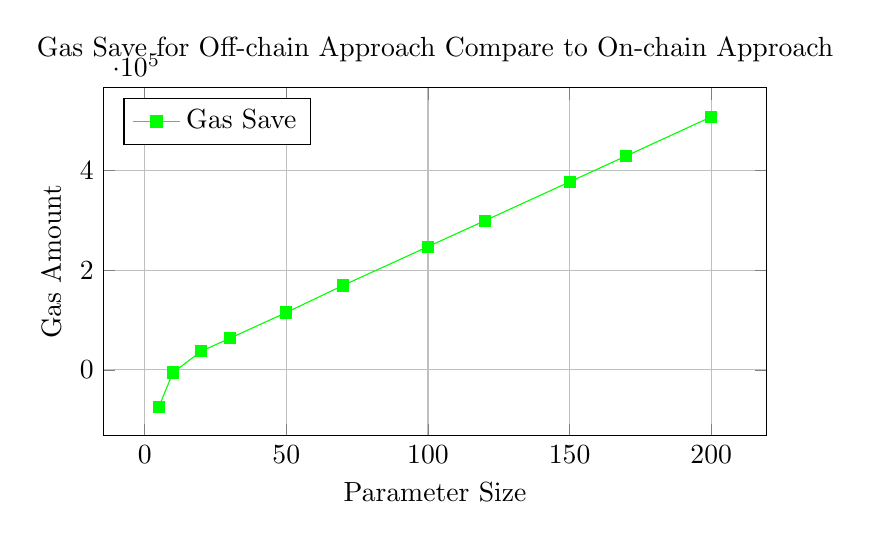
\begin{tikzpicture}
\label{gas-compare}
\begin{axis}[
    title={Gas Save for Off-chain  Approach Compare to On-chain Approach},
    xlabel={Parameter Size},
    ylabel={Gas Amount},
    legend pos=north west,
    grid=major,
    width=10cm,
    height=6cm
]

% Difference data
\addplot[
    color=green,
    mark=square*,
    ]
    coordinates {
    (5, -73971) (10, -5283) (20, 37754) (30, 63356) (50, 115328) (70, 169626) (100, 247493) (120, 299381) (150, 377536) (170, 429615) (200, 508057)
    };
    \addlegendentry{Gas Save}

\end{axis}
\end{tikzpicture}

\section{Related work}
\label{sec:related-work}
\section{Conclusion}
\label{sec:conclusion}
This paper proposes a method for parameter verification in smart contracts on the blockchain. The method addresses the challenge of performing computationally expensive verification processes directly on-chain. The core idea is to offload the verification process to an off-chain system, with only the verification results being submitted on-chain. To implement this approach, we propose an incentive mechanism that encourages validators to participate in the verification process while ensuring the correctness of the parameters when deemed valid. Our gas cost analysis demonstrates the benefits of this approach, particularly when dealing with large parameters that are costly to verify on-chain.
\newpage
\bibliographystyle{splncs04}
\bibliography{bio}
\end{document}
